\documentclass[a4paper,kul]{kulakarticle} %options: kul or kulak (default)

\usepackage[utf8]{inputenc}
\usepackage[english]{babel}
\usepackage{graphicx}
\usepackage{subcaption}
\newlength{\twosubht}
\newsavebox{\twosubbox}
\graphicspath{{../Figures/}{../Matlab/}{/}}
\usepackage[outdir=./]{epstopdf}

\usepackage{amsmath}
\usepackage{amsthm}
\usepackage{amssymb}
\usepackage{gensymb}
\setcounter{MaxMatrixCols}{21}

\usepackage{etoolbox,refcount}
\usepackage{multicol}

\newcounter{countitems}
\newcounter{nextitemizecount}
\newcommand{\setupcountitems}{%
	\stepcounter{nextitemizecount}%
	\setcounter{countitems}{0}%
	\preto\item{\stepcounter{countitems}}%
}
\makeatletter
\newcommand{\computecountitems}{%
	\edef\@currentlabel{\number\c@countitems}%
	\label{countitems@\number\numexpr\value{nextitemizecount}-1\relax}%
}
\newcommand{\nextitemizecount}{%
	\getrefnumber{countitems@\number\c@nextitemizecount}%
}
\newcommand{\previtemizecount}{%
	\getrefnumber{countitems@\number\numexpr\value{nextitemizecount}-1\relax}%
}
\makeatother    
\newenvironment{AutoMultiColItemize}{%
	\ifnumcomp{\nextitemizecount}{>}{3}{\begin{multicols}{2}}{}%
		\setupcountitems\begin{itemize}}%
		{\end{itemize}%
		\unskip\computecountitems\ifnumcomp{\previtemizecount}{>}{3}{\end{multicols}}{}}

\usepackage{pdflscape}

\date{Academic year 2021 -- 2022}
\address{
  Faculty of Engineering Science \\
  Department of Mechanical Engineering \\
  Control theory \texttt{[H04X3a]}}
\title{Report Assignment 1: Identification of the Motors}
\author{Matthias Derez, Toon Servaes}


\begin{document}

\maketitle

\tableofcontents
\listoffigures
\listoftables


\section{Model Structure}
\subsection{Discrete-time Model Structure} 
\label{subsec:complex_model}
In order to select the discrete-time model structure for the DC motors, the equivalent electric circuit in Figure \ref{fig:DCmotors} is used. By using Newton's second law and Kirchhoff's voltage law, following equations can be derived:

\begin{equation}
    \label{eq:circuit}
    \begin{split}
         J\ddot{\theta}  + b\dot{\theta} &= K_{t}i \\
         L\frac{di}{dt} + Ri &= V - K_{e}\dot{\theta}
     \end{split} 
\end{equation}
The meaning of each parameter is:
\begin{itemize}
    \item $J$ = moment of inertia of the rotor [kg $\cdot$ m$^2$]
    \item $\theta$ = angular position [rad]
    \item $\omega = \dot{\theta}$ = angular velocity [rad/s]
    \item $b$ = motor viscous friction constant [N $\cdot$ m $\cdot$ s]
    \item $K_{e}$ = electromotive force constant [$\frac{\text{V}}{\text{rad } \cdot \text{ s}}$] = $K_{t}$ = motor torque constant [$\frac{\text{N } \cdot \text{ m}}{\text{A }}$] = $K$
    \item $R$ = electric resistance [$\ohm$]
    \item $L$ = electric inductance [H]
\end{itemize}

\subsubsection*{Continuous-time Transfer Function}
Applying the Laplace transform to both equations in (\ref{eq:circuit}) leads to:

\begin{equation}
\begin{split}
	&Js^2\Theta(s) + bs\Theta(s) = KI(s) \\
	&LsI(s) + RI(s) = V(s) - Ks\Theta(s)	
\end{split}
\end{equation}
assuming $\theta(0) = 0$, $\dot{\theta}(0) = 0 \text{ and } i(0) = 0$. After some calculations, the continuous-time transfer function describing the behaviour of this system can be derived:
\begin{equation}
	\label{eq:TF}
    H(s) = \frac{\Omega(s)}{V(s)} = \frac{\dot{\Theta}(s)}{V(s)} = \frac{s\Theta(s)}{V(s)} = \frac{K}{(Js + b)(Ls + R) + K^2}
\end{equation}
where the input is the voltage source $V(s)$ applied to the motor's armature and the output is the rotational velocity of the wheel  $\dot{\Theta}(s)$. One can rewrite this transfer function in order to obtain a more general and well-known form:
\begin{equation}
\label{eq:TF2}
\begin{split}
	H(s) &= \frac{K}{(Js + b)(Ls + R) + K^2} \\
	 &= \frac{K}{LJs^2 + (Lb + JR)s + K^2 + bR} \\
	 &= \frac{\frac{K}{LJ}}{s^2 + \frac{Lb + JR}{LJ}s + \frac{K^2 + bR}{LJ}} \\
	 &= C \frac{\omega_n^2}{s^2 + 2\zeta\omega_ns + \omega_n^2}
\end{split}
\end{equation}
where $C = \frac{K}{K^2 + bR}$, $\omega_n^2 = \frac{K^2 + bR}{LJ}$ and $\zeta = \frac{Lb+JR}{2\sqrt{LJ(K^2 + bR)}}$.


\begin{figure}[htp!]
    \centering
    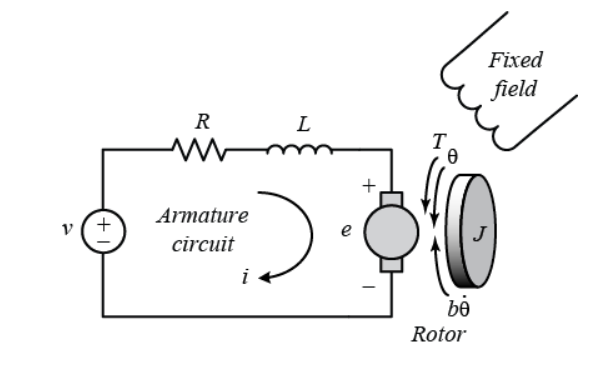
\includegraphics[width=.6\linewidth]{DC_motors.png}
    \caption[Electric circuit]{Electric equivalent circuit of the armature and the free-body diagram of the rotor.}
    \label{fig:DCmotors}
\end{figure}


\subsubsection*{Discrete-time Transfer Function}

The discrete-time transfer function is derived from the continuous-time one by using a zero-order hold sampling process. To this extent, one has to compute $H(z) = (1-z^{-1}) \mathcal{Z} (\mathcal{L}^{-1}\{\frac{H(s)}{s}\} \times \delta_T(t))$. The software running on the Arduino, called 'MicroOS', samples at $100$ Hz. Consequently, the sampling period $T_s = 0.01$ s. 
\\\\
Firstly, Equation (\ref{eq:TF2}) can be rewritten as follows: 
\begin{equation}
	H(s) = C \frac{\omega_n^2}{s^2 + 2\zeta\omega_ns + \omega_n^2} = C \frac{a^2 + b^2}{(s+a)^2 + b^2}
\end{equation}
where $a = \zeta\omega_n$ and $b = \sqrt{\omega_n^2(1-\zeta^2)}$. Next, using transform pair no. 22 on page 4 of the course formulary leads to:
\begin{equation}
	\mathcal{Z} \left(\mathcal{L}^{-1}\left\{\frac{H(s)}{s}\right\} \times \delta_T(t)\right) = C \frac{z(Az+B)}{(z-1)\left[z^2-2e^{-aT_s}\cos(bT_s)z+e^{-2aT_s}\right]}
\end{equation}
where $A = 1-e^{-aT_s}\cos(bT_s) - \frac{a}{b}e^{-aT_s}\sin(bT_s)$ and $B = e^{-2aT_s}\cos(bT_s) + \frac{a}{b}e^{-aT_s}\sin(bT_s) - e^{-aT_s}\cos(bT_s)$. Finally, the zero-order hold equivalent is determined:
\begin{equation}
	H(z) = (1-z^{-1})\mathcal{Z} \left(\mathcal{L}^{-1}\left\{\frac{H(s)}{s}\right\} \times \delta_T(t)\right) = C \frac{(Az+B)}{\left[z^2-2e^{-aT_s}\cos(bT_s)z+e^{-2aT_s}\right]}
\end{equation}
More generally: 
\begin{equation}
	H(z) = \frac{b_0z + b_1}{z^2 + a_0 z + a_1}
\end{equation}
However, the MicroOS software on the Arduino stores the control command calculated during discrete-time interval $k$ in a memory buffer until discrete-time instance $k+1$. In this way, the delay between the measurement of the output and sending out of the control command is increased by one sampling period $T_s$. In the $z$-domain, this is equivalent to a multiplication of the transfer function by $z^{-1}$, leading to the final, generalised discrete-time transfer function of the system:
\begin{equation}
	\label{eq:TF3}
	H(z) = \frac{b_0z + b_1}{z^3 + a_0 z^2 + a_1 z}
\end{equation}
The ZOH discretization leads to an input delay of approximately $\frac{T_s}{2}$. Together with the delay introduced by the MicroOS software, the effective delay amounts to $\frac{3T_s}{2}$. Because the input and output data are observed at discrete time instances, a change in the input voltage is observed in the output $\lceil \frac{3}{2} \rceil T_s = 2T_s$ seconds, or equivalently, 2 time instances (samples) later. This is verified by Figure \ref{fig:delay}, where the input voltage sent to motor A changes at $t = 0.01$s, while the velocity changes at $t = 0.03$s. \\
\noindent In the final transfer function (\ref{eq:TF3}), the order of the numerator is 1, while the order of the denominator is 3. This is in line with the strict causality condition, which demands that the order of the numerator is strictly smaller than the denominator. 

\begin{figure}
	\centering
	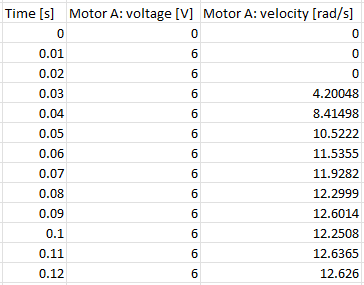
\includegraphics[width=.5\linewidth]{delay.png}
	\caption[Data snippet]{Snippet of the recorded data showing the delay between the input voltage and the motor velocity change.}
	\label{fig:delay}
\end{figure}


% ---------------------------------------------------------------------------
\subsection{Simplified Model}
Another, simplified model is also examined. The reason for this is that equally accurate results may be achieved using simpler equations. This simplified model is achieved by neglecting the inductance term in Equation \ref{eq:TF}, because its effect is several times smaller in comparison with the mechanical terms. This leads to:
\begin{equation}
\label{eq:TF_simple}
	\begin{split}
	H_{\text{simple}}(s) &= \frac{K}{JRs + (bR + K^2)} \\
	&= \frac{\frac{K}{JR}}{s + \frac{bR + K^2}{JR}} \\
	&= \frac{1}{C}\frac{a}{s + a}
	\end{split}
\end{equation}
where $C = \frac{K}{K^2 + bR}$, which is the same as in Equation \ref{eq:TF2}. Now, transform pair no. 12 leads to the zero-order hold equivalent of this simplified model:
\begin{equation}
	H_{\text{simple}}(z) = \frac{1}{C}\frac{1-e^{-aT_s}}{z-e^{-aT_s}}
\end{equation}
More generally:
\begin{equation}
	H_{\text{simple}}(z) = \frac{b_0}{z + a_0}
\end{equation}
Again, the extra delay is taken into account, resulting in the final, simplified, discrete-time transfer function of the system:
\begin{equation}
\label{eq:TF_simple2}
	H_{\text{simple}}(z) = \frac{b_0}{z^2 + a_0 z}
\end{equation}

\noindent Now, the order of the numerator is 0 and of the denominator 2. This means that the strict causality condition is again satisfied, while there is also a delay of 2 samples between input and output.
\\\\
Both the transfer functions of the complex model (\ref{eq:TF3}) and the simple model (\ref{eq:TF_simple2}) are used in the rest of the assignment. The unknown parameters $b_0$, $b_1$, $a_0$ and $a_1$ are determined in Section \ref{subsec:lse} using the least-squares method. This is done for each motor separately. Then, depending on which model gives the best results, either the complex or the simple model is chosen.
\\\\
From now on, the original model of Subsection \ref{subsec:complex_model} is referred to as the \textit{complex model} and this simplified model as \textit{simple model}.





% ---------------------------------------------------------------------------

\subsection{Input and Output}
As previously mentioned, the input of the model is the voltage source $V(s)$ applied to the motor's armature. This voltage is controlled by the Arduino and is expressed in Volts [V]. The output is the rotational velocity of the wheel  $\Omega(s) = \dot{\Theta}(s)$, expressed in [rad/s].

% ---------------------------------------------------------------------------

\section{Identification of each 'DC Motor + Wheel'}
\subsection{Excitation Signal}
In order to identify the system 'DC motor + wheel', it is necessary to perform a dedicated experiment that actively excites the system, while the \textit{persistency of excitation} condition is satisfied. This means that the excitation must be rich enough, i.e. so that all frequency modes of the system are excited and observable in the output. To this extent, a square wave is chosen, as displayed in Figure \ref{fig:IO} on the left. Note that the input voltage also remains $0$ for some time, instead of jumping to $-6$ or $6$ instantaneously. 
\\\\
This step-up step-down pattern is repeated four times in order to assess the noise and to check wether modelling errors increase throughout repition of the periods. In Figure \ref{fig:omega_deltaomega}, the top plots show the motor velocities averaged out to one period of the square wave excitation. The bottom plots show the deviation of the motor velocities with regard to the averaged out velocities, for each of the periods (each with a different colour). The left plots are for motor A and the right ones for motor B. One can see that the motor velocities fluctuate not more than $\pm 3.5\%$, which is acceptable to work with for the rest of the assignment. There is no noise on the input voltage, as it is controlled by the user.

\begin{figure*}[htp!]
	\centering
	\begin{subfigure}[b]{0.485\textwidth}
		\centering
		\includegraphics[width=\textwidth]{input_voltage.eps}
	\end{subfigure}
	\hfill
	\begin{subfigure}[b]{0.5\textwidth}  
		\centering 
		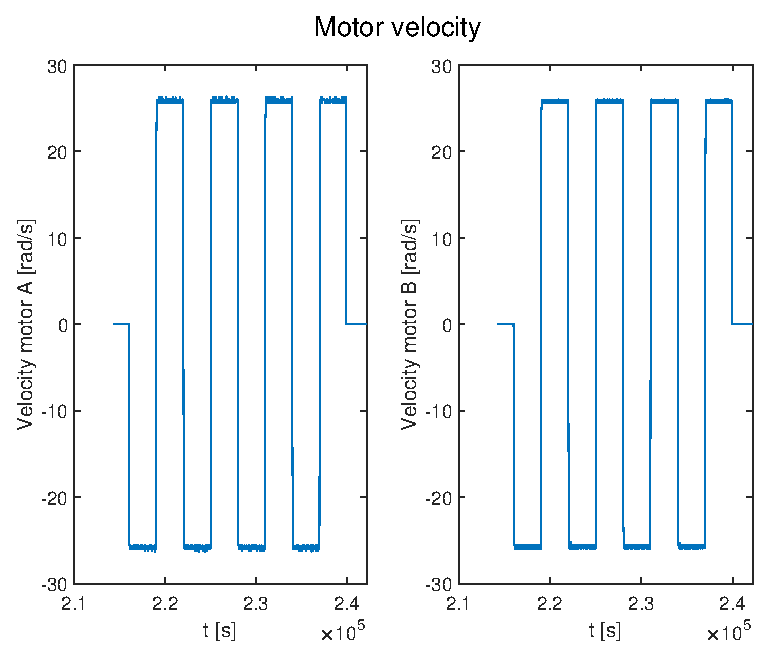
\includegraphics[width=\textwidth]{motor_velocity.eps}
	\end{subfigure}
	\caption[Input voltage \& Motor velocity]{\textbf{Left}: Input voltage [V]. \textbf{Right}: Motor velocities [rad/s], for motor A and B respectively.} 
	\label{fig:IO}
\end{figure*}

\begin{figure*}[htp!]
	\centering
	\begin{subfigure}[b]{0.49\textwidth}
		\centering
		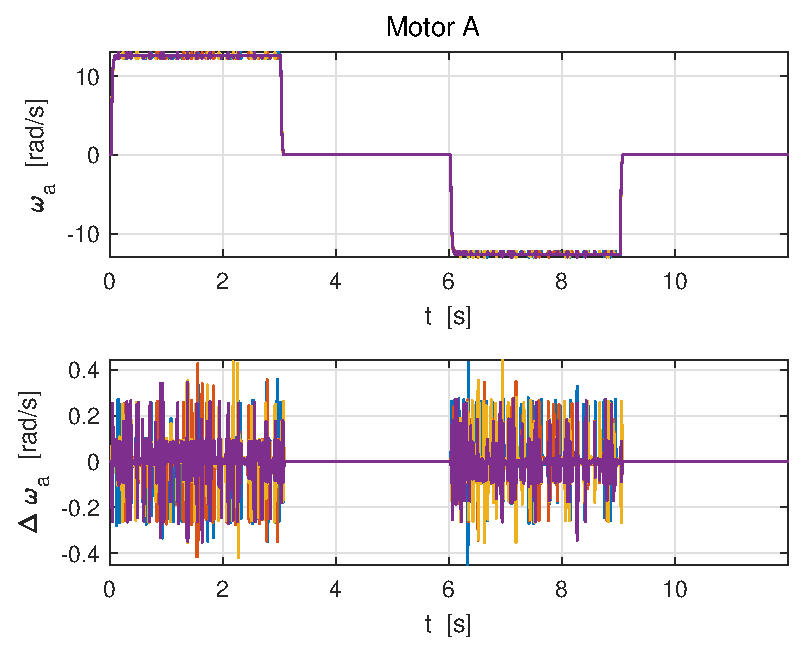
\includegraphics[width=\textwidth]{omegaA_deltaomegaA.eps}
	\end{subfigure}
	\hfill
	\begin{subfigure}[b]{0.49\textwidth}  
		\centering 
		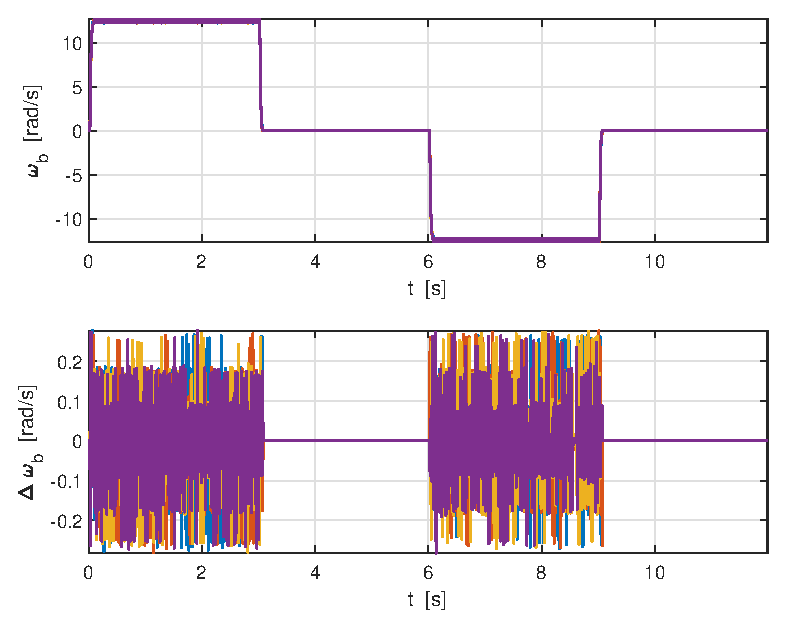
\includegraphics[width=\textwidth]{omegaB_deltaomegaB.eps}
	\end{subfigure}
	\caption[Average velocity]{\textbf{Top}: Motor velocities averaged out to one period of the square wave excitation. \textbf{Bottom}: Deviation of the motor velocities with regard to the averaged out velocities, for each of the periods.} 
	\label{fig:omega_deltaomega}
\end{figure*}

% ---------------------------------------------------------------------------

\subsection{System Parameters}
\label{subsec:lse}
\subsubsection{Estimation criterion}

Now, the unknown parameters $b_0$, $b_1$, $a_0$ and $a_1$ of Equations \ref{eq:TF3} and \ref{eq:TF_simple2} are determined for each motor. This is done using the least squares method where the \textit{least squares criterion} is minimized: 
\begin{equation}
	\label{eq:lse}
	\text{min } V_N (\vec{\theta}, \vec{Z}^N) = \text{min }\sum_{t = 1}^{N}\frac{1}{2} \left[\omega[t] - \vec{\phi}^{\text{ }T}[t]\vec{\theta}\right]^2
\end{equation}
where $\vec{\theta}$ is \textbf{not} the angular position of the wheels, but a vector composed of the unknown coefficients, $\vec{Z}^N$ is the measured input and output data and $\vec{\phi}[t]$ is a vector containing the coefficients of the difference equation. Equation \ref{eq:lse} boils down to minimizing the squared error between the empirical output and the estimated output. 


\subsubsection*{Complex Model}
The difference equation of the complex model is derived as follows:
\begin{equation}
\begin{split}
\frac{\Omega(z)}{V(z)} &= \frac{b_0z + b_1}{z^3 + a_0 z^2 + a_1 z} \\
\iff (1 + a_0 z^{-1} + a_1 z^{-2})\Omega(z) &= (b_0 z^{-2} + b_1 z^{-3})V(z) \\
\iff \omega[t] + a_0 \omega[t-1] + a_1 \omega[t-2] &= b_0 V[t-2] + b_1 V[t-3] 
\end{split}
\end{equation}
This means that:
\begin{equation}
\begin{split}
\vec{\theta} &= \left[a_0\text{ }a_1\text{ }b_0\text{ }b_1\right]^T \\
\vec{\phi}[t] &= \left[-\omega[t-1]\text{ }-\omega[t-2]\text{ }V[t-2]\text{ }V[t-3]\right]^T
\end{split}
\end{equation}


\subsubsection*{Simple Model}
Analogously for the simple model:
\begin{equation}
\begin{split}
\frac{\Omega(z)}{V(z)} &= \frac{b_0}{z^2 + a_0 z} \\
\iff (1 + a_0 z^{-1})\Omega(z) &= b_0 z^{-2} V(z) \\	
\iff \omega[t] + a_0 \omega[t-1] &= b_0 V[t-2]
\end{split}
\end{equation}
This yields: 
\begin{equation}
\begin{split}
\vec{\theta}_{\text{simple}} &= \left[a_0\text{ }b_0\right]^T \\
\vec{\phi}[t]_{\text{simple}} &= \left[-\omega[t-1]\text{ }V[t-2]\right]^T
\end{split}
\end{equation}

\subsubsection{Results}
\noindent The unknown coefficients are determined using \texttt{Matlab}. This allows to construct the transfer function for each of the motors, as well as the locations of the poles and the zeros. These values are summarized in Table \ref{tab:overview} and visualized in Figures \ref{fig:pz_complex_all} and \ref{fig:pz_simple_all}.
\\\\
As expected, the simple model has no zeros, because the numerator of the transfer function is of order 0. The NaN values (in rad/s) in the table refer to the poles that are at the origin of the pole-zero map. Both models have such a pole, because of the multiplication by $z^{-1}$ to take the MicroOS delay into account. 

% Further, for the simple model, the transfer functions for motor A and B are approximately the same, which explains why the poles for motor A and B coincide in Figure \ref{fig:pz_simple}.

% @Matthias: hier stond aanvankelijk de tabel, toen de pzmap er ook stond.


%\begin{figure*}[htp!]
%	\centering
%	\begin{subfigure}[b]{0.48\textwidth}
%		\centering
%		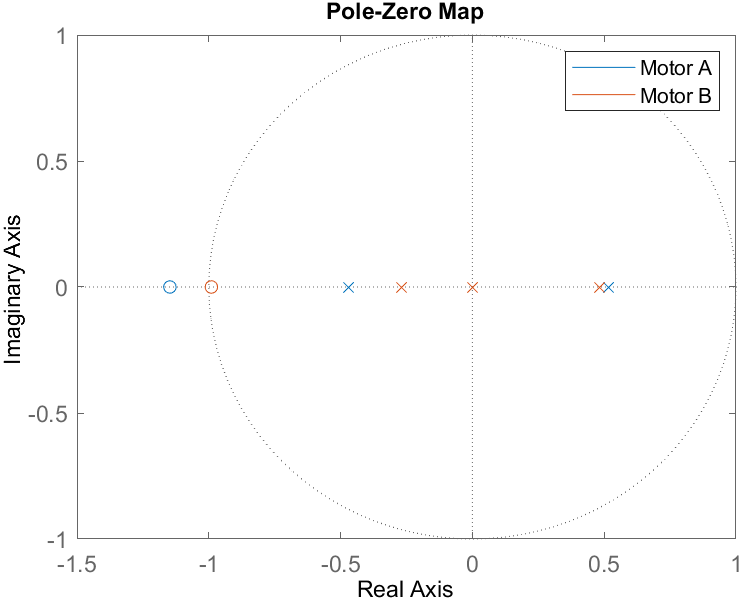
\includegraphics[width=\textwidth]{p&z_complex_cropped.pdf}
%		\caption{\textbf{Complex} model}
%	\end{subfigure}
%	\hfill
%	\begin{subfigure}[b]{0.48\textwidth}  
%		\centering 
%		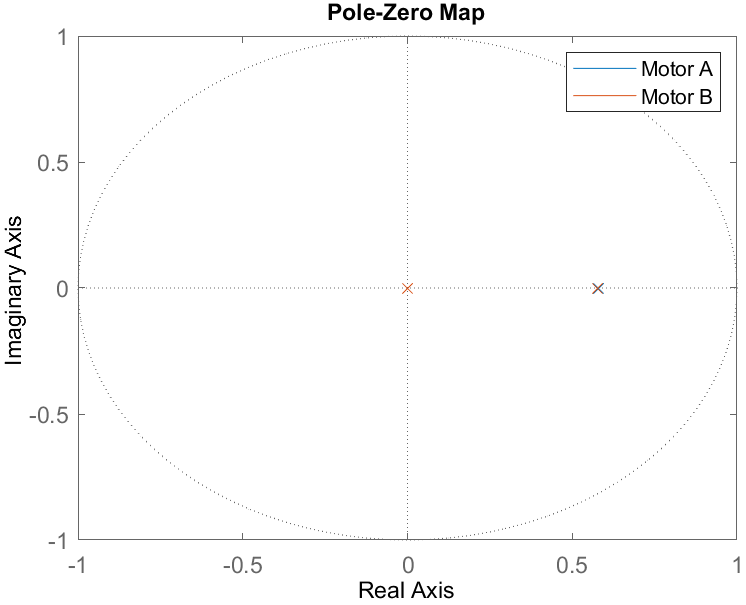
\includegraphics[width=\textwidth]{p&z_simple_cropped.pdf}
%		\caption{\textbf{Simple} model}
%		\label{fig:pz_simple}
%	\end{subfigure}
%	\caption{Visualization of the poles and the zeros of both models, for each motor.} 
%	\label{fig:pz}
%\end{figure*}



% ---------------------------------------------------------------------------

\subsection{Filtering}
In the least-squares ARX model parameter estimation, the quadratic prediction error emphasises errors at high frequencies. Because noisy data typically resides at these high frequencies, low-pass data filtering can be used to improve the parameter estimation. The input data is free of noise, because it is controlled by the user. However, if one would only filter the output data, one would not only identify the physical system, but also the filter. This is why both input \textbf{and} output data are filtered. 

\subsubsection{Butterworth Filter}
\label{subsub:BW}

First, a low-pass Butterworth filter is examined. The order of the filter is chosen higher than the system in order to have more flexibility and to have a strong enough attenuation of high frequencies. On the other hand, the order may not be too high, otherwise both input and output data have a big delay. In this manner, a $6^{\text{th}}$ order filter is used. 
\\\\
In addition, the cut-off frequency must be smaller than half the sample rate. Normally, the cut-off is determined as the frequency where the magnitude of the \textbf{exact} model is equal to 3 dB. Though, the exact model of the system is not known, so the cut-off is approximated by the bandwidth of the unfiltered identified model of Table \ref{tab:overview}. 
%In Subsection \ref{subsec:validation}, this cut-off is further optimised in order to minimize the error between the identified model and the empirical values.
\\\\
Table \ref{tab:overview_BW} summarizes the identification after applying the filter. For the complex model, the poles are a lot smaller than without the filter. This means that the modelled system reacts much slower, which is not desirable. On the other hand, for the simple model, the poles are a bit greater, leading to a faster responding system. One can conclude that the filtering is only beneficial when using the simple system.


% @Matthias: hier stond aanvankelijk de tabel, toen de pzmap er ook stond.



%\begin{figure*}[htp!]
%	\centering
%	\begin{subfigure}[b]{0.48\textwidth}
%		\centering
%		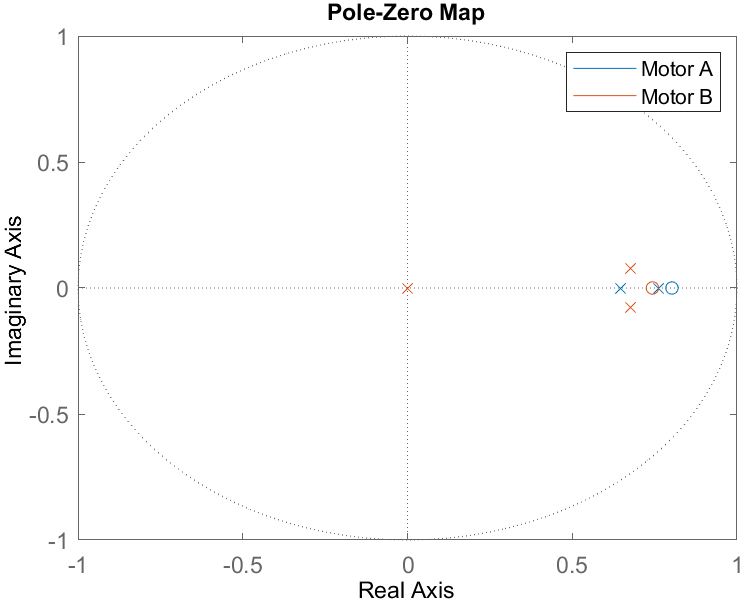
\includegraphics[width=\textwidth]{p&z_complex_BW_cropped.pdf}
%		\caption{\textbf{Complex} model}
%	\end{subfigure}
%	\hfill
%	\begin{subfigure}[b]{0.48\textwidth}  
%		\centering 
%		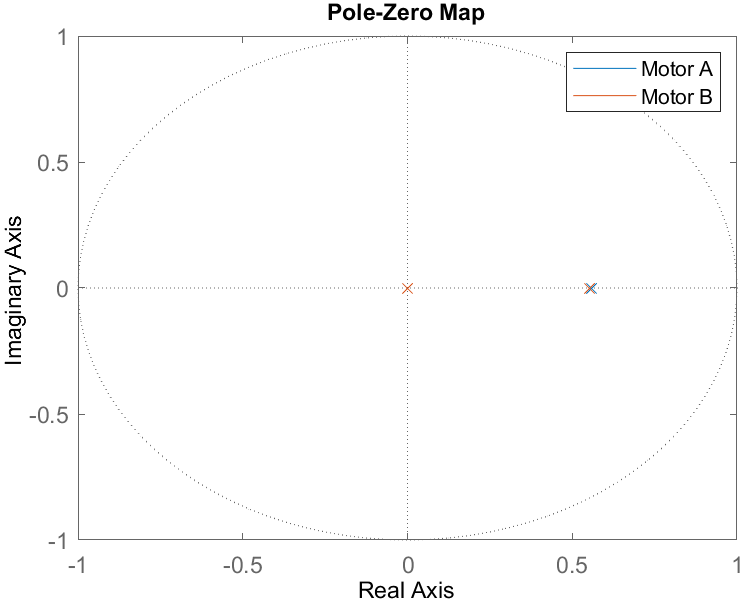
\includegraphics[width=\textwidth]{p&z_simple_BW_cropped.pdf}
%		\caption{\textbf{Simple} model}
%		\label{fig:pz_simple_BW}
%	\end{subfigure}
%	\caption{Visualization of the poles and the zeros of both models, after applying a \textbf{Butterworth} filter.} 
%	\label{fig:pz_BW}
%\end{figure*}


\subsubsection{Sanathanan Koerner Filter}

As the results from \ref{subsub:BW} are not that fantastic, another filtering procedure is examined. It is an iterative weighted least-square approach, called the Sanathanan Koerner procedure. In this technique, the model without filter is used as starting point. In each iteration step i, the obtained model is filtered with a low-pass filter given by 1 divided by the denominator of the obtained model of step i-1. This goes on until the denominator of the obtained model of step i-1 comes arbitrarily close to the denominator of step i. This way, the high-frequency emphasis introduced in the obtained model will be completely compensated. In this report, convergence is assumed when the error between the denominators reaches machine precision.
\\\\
The results of the identification are given in Table \ref{tab:overview_SK}. When compared to Table \ref{tab:overview}, one can observe that the poles for both motors are almost equally fast or even faster than without filter, and this for \textbf{both models}. Comparing to Table \ref{tab:overview_BW} shows that the poles are a bit slower for the simple model, but a lot faster for the complex model.
\\\\
From this analysis, one can deduce that the Sanathanan Koerner filter procedure is the way to go. The poles and zeros of all the models are again visualized in Figures \ref{fig:pz_complex_all} and \ref{fig:pz_simple_all}.

\begin{table}[htp]
	\centering
	\caption{Overview of the complex and simple models for each motor.}
	\label{tab:overview}
	\bgroup
	\def\arraystretch{1.8}
	\begin{tabular}{|c||cc||cc|}
		\hline & \multicolumn{2}{c||}{\textbf{Complex}} & \multicolumn{2}{c|}{\textbf{Simple}} 
		\\ \hline \hline
		& \multicolumn{1}{c|}{Motor A} & Motor B & \multicolumn{1}{c|}{Motor A} & Motor B
		\\ \hline
		Transfer function & \multicolumn{1}{c|}{\scalebox{1.15}{$\frac{0.6952\text{ }z + 0.7978}{z^3 - 0.04632\text{ }z^2 - 0.242\text{ }z}$}} & \scalebox{1.15}{$\frac{0.6901\text{ }z + 0.6834}{z^3 - 0.2128\text{ }z^2 - 0.1303\text{ }z}$} & \multicolumn{1}{c|}{\scalebox{1.15}{$\frac{ 0.8842}{z^2 - 0.5787\text{ }z}$}} & \scalebox{1.15}{$\frac{0.8832}{z^2 - 0.5778\text{ }z}$} 
		\\ \hline
		Poles [rad/s] & \multicolumn{1}{c|}{66.2; 323; NaN} & 72.8; 340; NaN & \multicolumn{1}{c|}{54.7; NaN} & 54.9; NaN
		\\ \hline
		Zeros [rad/s] & \multicolumn{1}{c|}{314} & 314 & \multicolumn{1}{c|}{/} & /
		\\ \hline
	\end{tabular}
	\egroup
\end{table}

\begin{table}[htp]
	\centering
	\caption[Overview of the complex and simple models, after applying a Butterworth filter]{Overview of the complex and simple models, after applying a \textbf{Butterworth} filter.}
	\label{tab:overview_BW}
	\bgroup
	\def\arraystretch{1.8}
	\begin{tabular}{|c||cc||cc|}
		\hline & \multicolumn{2}{c||}{\textbf{Complex}} & \multicolumn{2}{c|}{\textbf{Simple}} 
		\\ \hline \hline
		& \multicolumn{1}{c|}{Motor A} & Motor B & \multicolumn{1}{c|}{Motor A} & Motor B
		\\ \hline
		Cut-off [Hz] & \multicolumn{1}{c|}{10.7482} & 11.5228 & \multicolumn{1}{c|}{8.9104} & 8.9370
		\\ \hline
		Transfer function & \multicolumn{1}{c|}{\scalebox{1.15}{$\frac{0.8998\text{ }z - 0.7222}{z^3 - 1.407\text{ }z^2 + 0.4917\text{ }z}$}} & \scalebox{1.15}{$\frac{0.8989\text{ }z - 0.6683}{z^3 - 1.354\text{ }z^2 + 0.4644\text{ }z}$} & \multicolumn{1}{c|}{\scalebox{1.15}{$\frac{0.9284}{z^2 - 0.5576\text{ }z}$}} & \scalebox{1.15}{$\frac{0.9393}{z^2 - 0.5509\text{ }z}$} 
		\\ \hline
		Poles [rad/s] & \multicolumn{1}{c|}{27.4; 43.6; NaN} & 40; 40; NaN & \multicolumn{1}{c|}{58.4; NaN} & 59.6; NaN
		\\ \hline
		Zeros [rad/s] & \multicolumn{1}{c|}{22} & 29.6 & \multicolumn{1}{c|}{/} & /
		\\ \hline
	\end{tabular}
	\egroup
\end{table}

\begin{table}[htp]
	\centering
	\caption[Overview of the complex and simple models, after the Sanathanan Koerner filter]{Overview of the complex and simple models, after the \textbf{Sanathanan Koerner} filter procedure.}
	\label{tab:overview_SK}
	\bgroup
	\def\arraystretch{1.8}
	\begin{tabular}{|c||cc||cc|}
		\hline & \multicolumn{2}{c||}{\textbf{Complex}} & \multicolumn{2}{c|}{\textbf{Simple}} 
		\\ \hline \hline
		& \multicolumn{1}{c|}{Motor A} & Motor B & \multicolumn{1}{c|}{Motor A} & Motor B
		\\ \hline
		Transfer function & \multicolumn{1}{c|}{\scalebox{1.15}{$\frac{0.7124\text{ }z + 0.8249}{z^3 - 0.004181\text{ }z^2 - 0.2714\text{ }z}$}} & \scalebox{1.15}{$\frac{0.6884\text{ }z + 0.636}{z^3 - 0.2687\text{ }z^2 - 0.09782\text{ }z}$} & \multicolumn{1}{c|}{\scalebox{1.15}{$\frac{ 0.9158}{z^2 - 0.5636\text{ }z}$}} & \scalebox{1.15}{$\frac{0.9249}{z^2 - 0.5578\text{ }z}$} 
		\\ \hline
		Poles [rad/s] & \multicolumn{1}{c|}{65.6; 321; NaN} & 74.5; 352; NaN & \multicolumn{1}{c|}{57.3; NaN} & 58.4; NaN
		\\ \hline
		Zeros [rad/s] & \multicolumn{1}{c|}{315} & 314 & \multicolumn{1}{c|}{/} & /
		\\ \hline
	\end{tabular}
	\egroup
\end{table}

%\begin{figure*}[htp!]
%	\centering
%	\begin{subfigure}[b]{0.48\textwidth}
%		\centering
%		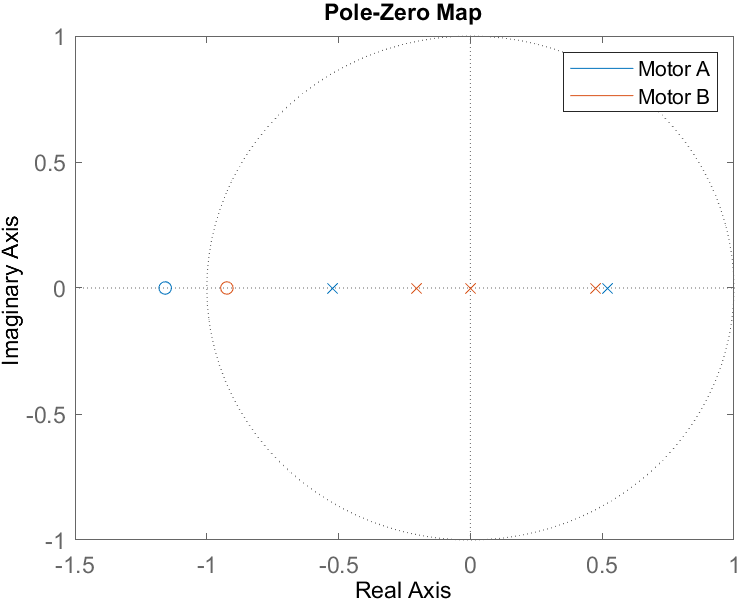
\includegraphics[width=\textwidth]{p&z_complex_SK_cropped.pdf}
%		\caption{\textbf{Complex} model}
%	\end{subfigure}
%	\hfill
%	\begin{subfigure}[b]{0.48\textwidth}  
%		\centering 
%		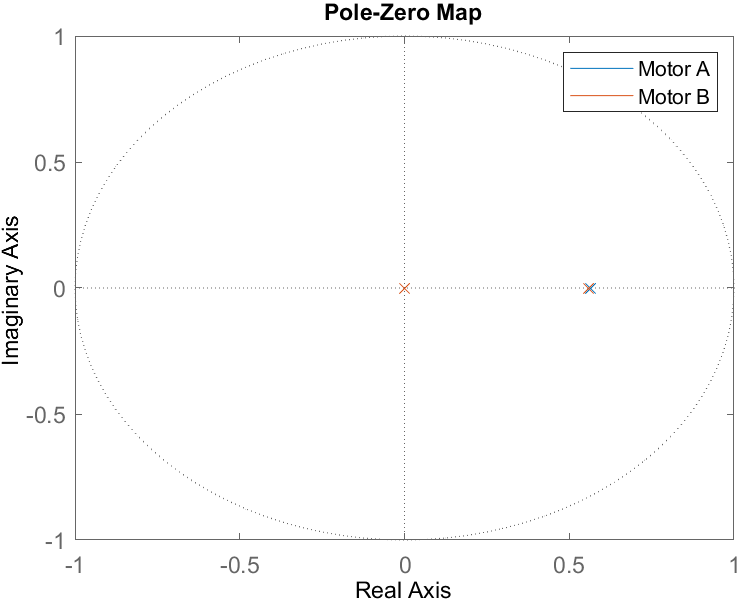
\includegraphics[width=\textwidth]{p&z_simple_SK_cropped.pdf}
%		\caption{\textbf{Simple} model}
%		\label{fig:pz_simple_SK}
%	\end{subfigure}
%	\caption{Visualization of the poles and the zeros of both models, after applying the \textbf{Sanathanan Koerner} filter procedure.} 
%	\label{fig:pz_SK}
%\end{figure*}

\newpage

\begin{figure*}[htp!]
	\centering
	\begin{subfigure}[b]{0.48\textwidth}
		\centering
		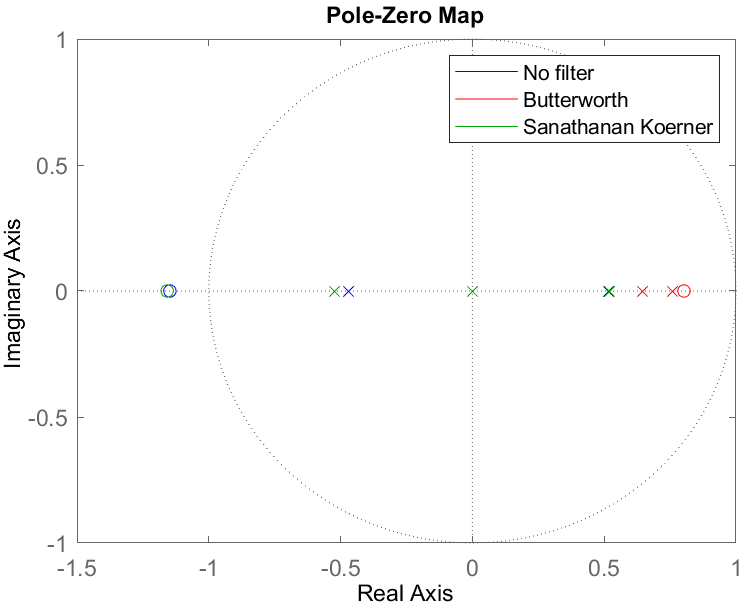
\includegraphics[width=\textwidth]{p&z_complex_all_A_cropped.pdf}
		\caption{Motor A}
	\end{subfigure}
	\hfill
	\begin{subfigure}[b]{0.48\textwidth}  
		\centering 
		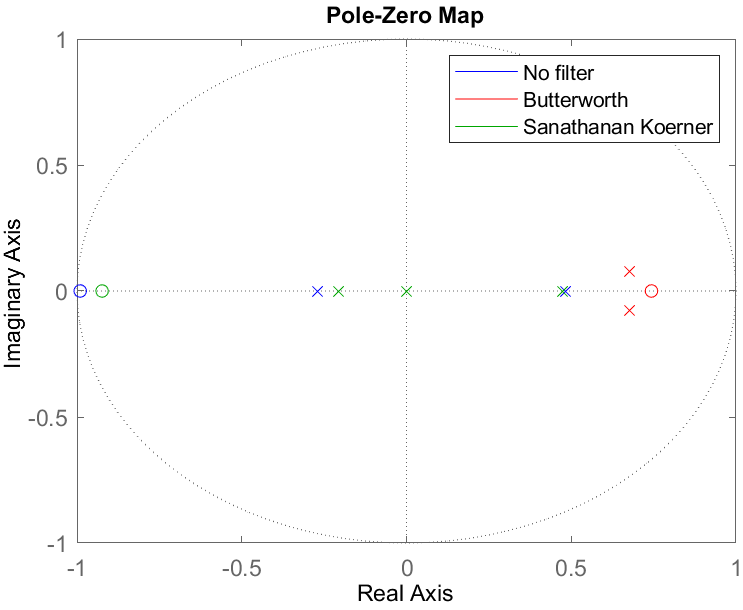
\includegraphics[width=\textwidth]{p&z_complex_all_B_cropped.pdf}
		\caption{Motor B}
	\end{subfigure}
	\caption[Pole-Zero map complex model]{Visualization of the poles and the zeros for the \textbf{complex} model without filter, with Butterworth filter and with Sanathanan Koerner filter.} 
	\label{fig:pz_complex_all}
\end{figure*}

\begin{figure*}[htp!]
	\centering
	\begin{subfigure}[b]{0.48\textwidth}
		\centering
		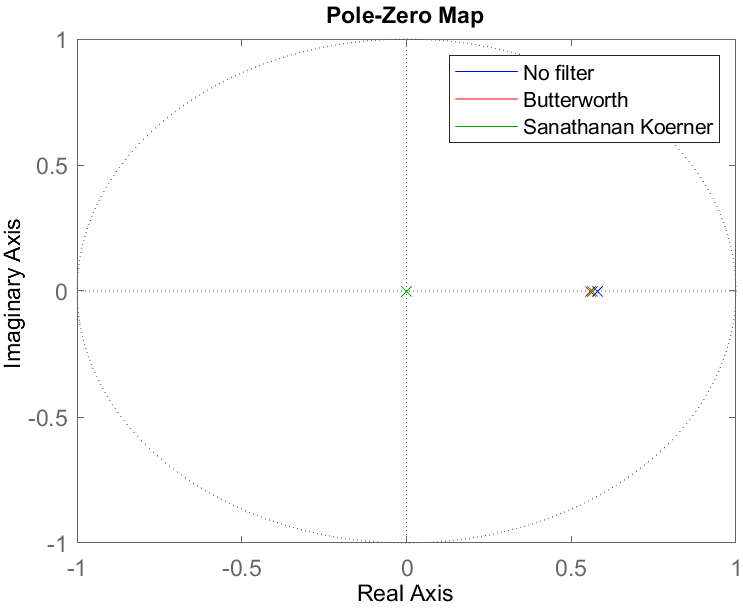
\includegraphics[width=\textwidth]{p&z_simple_all_A_cropped.pdf}
		\caption{Motor A}
	\end{subfigure}
	\hfill
	\begin{subfigure}[b]{0.48\textwidth}  
		\centering 
		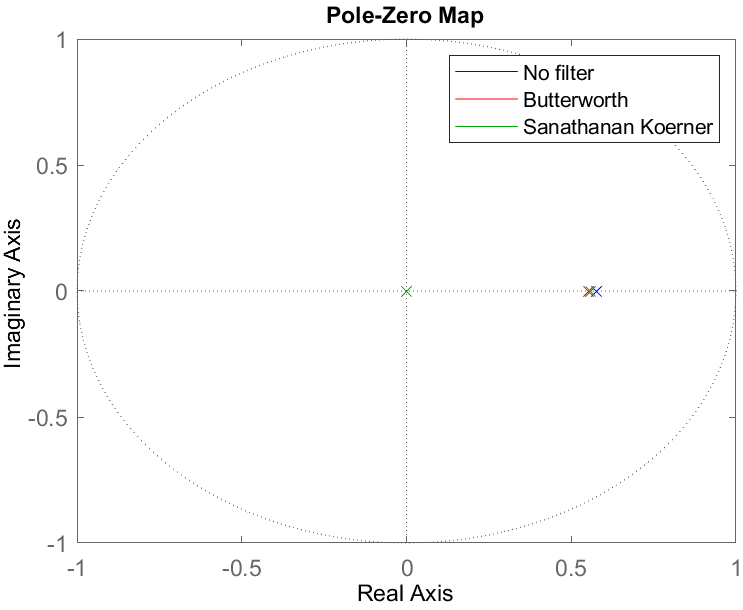
\includegraphics[width=\textwidth]{p&z_simple_all_B_cropped.pdf}
		\caption{Motor B}
	\end{subfigure}
	\caption[Pole-Zero map simple model]{Visualization of the poles and the zeros for the \textbf{simple} model without filter, with Butterworth filter and with Sanathanan Koerner filter.} 
	\label{fig:pz_simple_all}
\end{figure*}





% ---------------------------------------------------------------------------

\subsection{Experimental Model Validation}
\label{subsec:validation}

\subsubsection{Estimated vs. empirical Results}

This Subsection examines the simulated response to a step input for each of the identified models. This response is then compared to the empirical response, in order to judge the accuracy of the models. Figure \ref{fig:validation_complex} displays the results for the complex models and Figure \ref{fig:validation_simple} for the simple models. 
\\\\
First and foremost, the plots clearly show that the models using a Butterworth filter are worse than the models with no filter. Next, there is very little difference between the models with Sanathanan Koerner filtering and the models without filter. Adding complexity without having major improvements is unnecessary, so the unfiltered models are preferred.
\\\\
Lastly, comparing Figures \ref{fig:validation_complex} and \ref{fig:validation_simple} indicates that there is a trade-off between accuracy and model complexity. However, for both motors, the performance improvement is too small to justify using a more complex model. Conclusion: the simple, unfiltered models are preferred for both motors.
\begin{figure*}[htp!]
	\centering
	\begin{subfigure}[b]{0.48\textwidth}
		\centering
		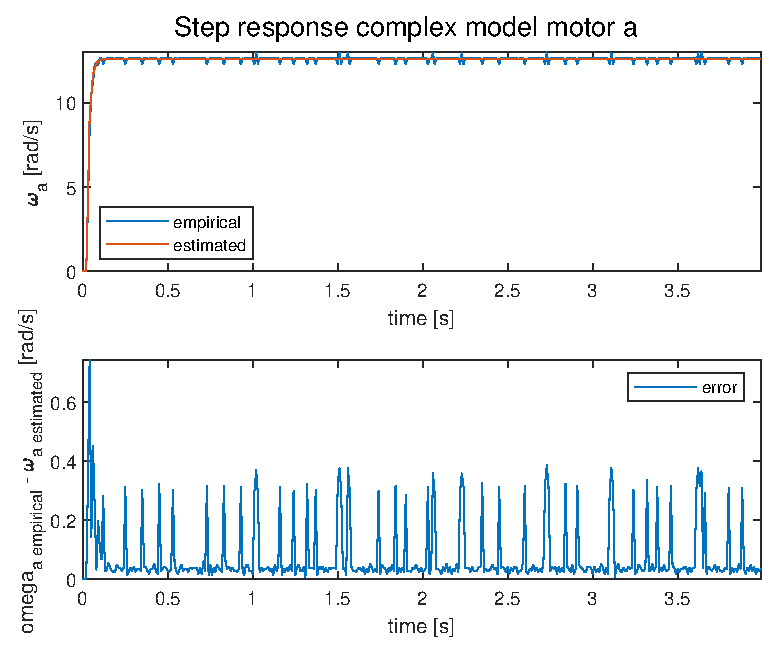
\includegraphics[width=\linewidth]{step_response_complex_a.eps}
	\end{subfigure}
	\hfill
	\begin{subfigure}[b]{0.48\textwidth}
		\centering
		\includegraphics[width=\linewidth]{step_response_complex_b.eps}
	\end{subfigure}
	\par\bigskip
	\begin{subfigure}[b]{0.48\textwidth}
		\centering
		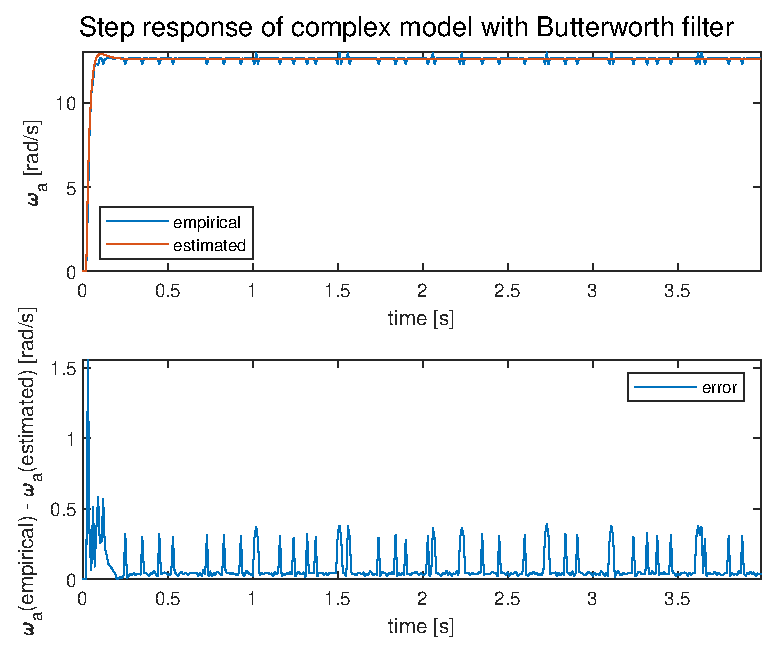
\includegraphics[width=\linewidth]{step_response_complex_BW_a.eps}
	\end{subfigure}
	\hfill
	\begin{subfigure}[b]{0.48\textwidth}
		\centering
		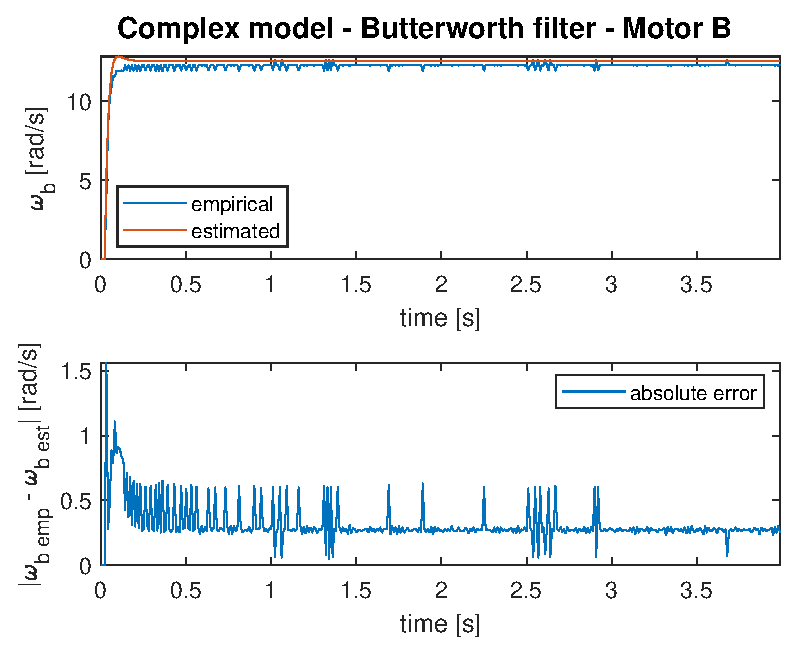
\includegraphics[width=\linewidth]{step_response_complex_BW_b.eps}
	\end{subfigure}
	\par\bigskip
	\begin{subfigure}[b]{0.48\textwidth}
		\centering
		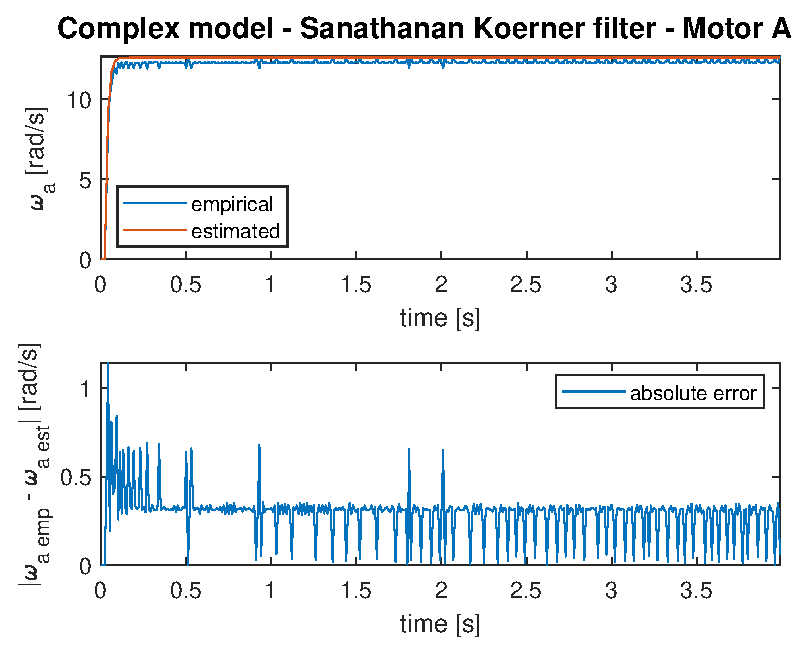
\includegraphics[width=\linewidth]{step_response_complex_SK_a.eps}
	\end{subfigure}
	\hfill
	\begin{subfigure}[b]{0.48\textwidth}
		\centering
		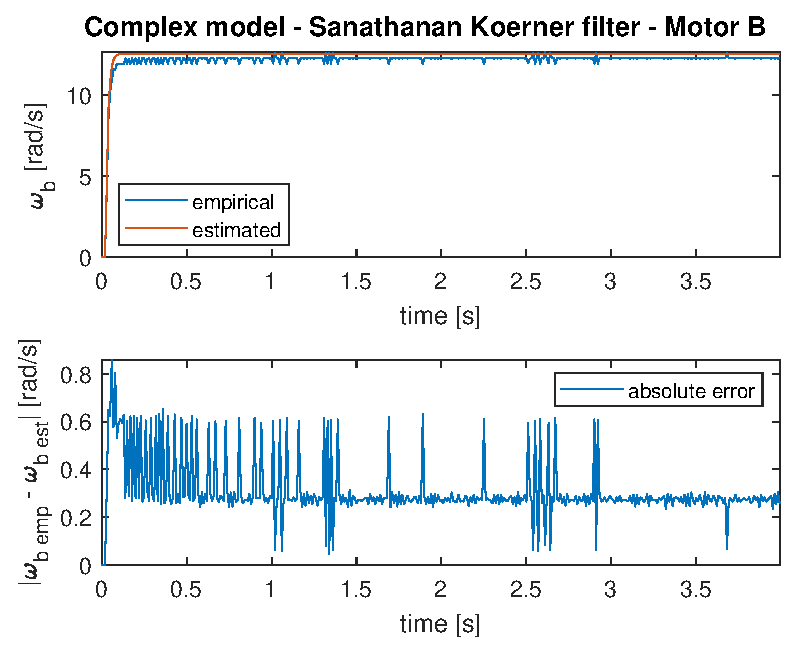
\includegraphics[width=\linewidth]{step_response_complex_SK_b.eps}
	\end{subfigure}
	\caption[Experimental results for the complex models]{Experimental results for the \textbf{complex} models: without filter, with Butterworth and with Sanathanan Koerner. The left side concerns motor A, while the right side concerns motor B. There are two types of plots: the top one always expresses the wheel velocity, while the bottom one indicates the absolute error between the empirical wheel velocity and the velocity predicted by the model.}
	\label{fig:validation_complex}
\end{figure*}

\begin{figure*}[htp!]
	\centering
	\begin{subfigure}[b]{0.48\textwidth}
		\centering
		\includegraphics[width=\linewidth]{step_response_simple_a.eps}
	\end{subfigure}
	\hfill
	\begin{subfigure}[b]{0.48\textwidth}
		\centering
		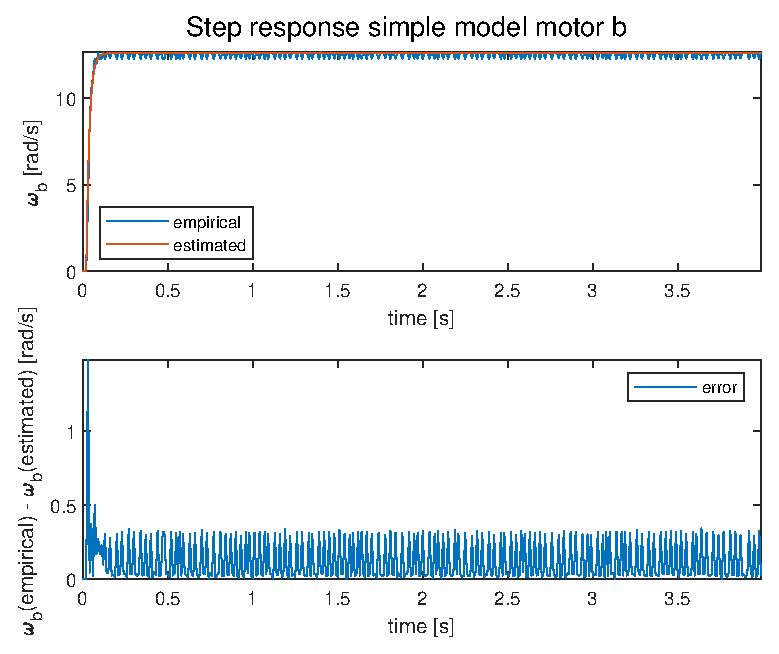
\includegraphics[width=\linewidth]{step_response_simple_b.eps}
	\end{subfigure}
	\par\bigskip
	\begin{subfigure}[b]{0.48\textwidth}
		\centering
		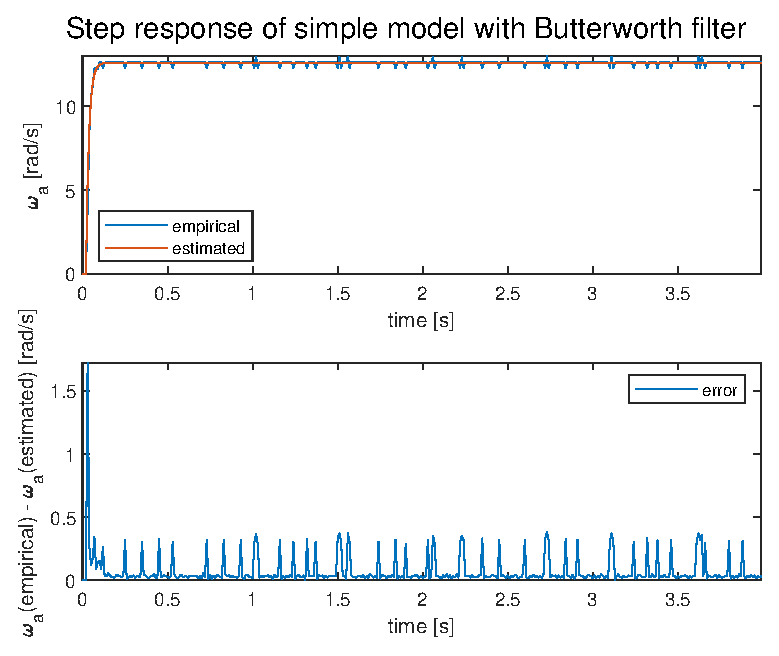
\includegraphics[width=\linewidth]{step_response_simple_BW_a.eps}
	\end{subfigure}
	\hfill
	\begin{subfigure}[b]{0.48\textwidth}
		\centering
		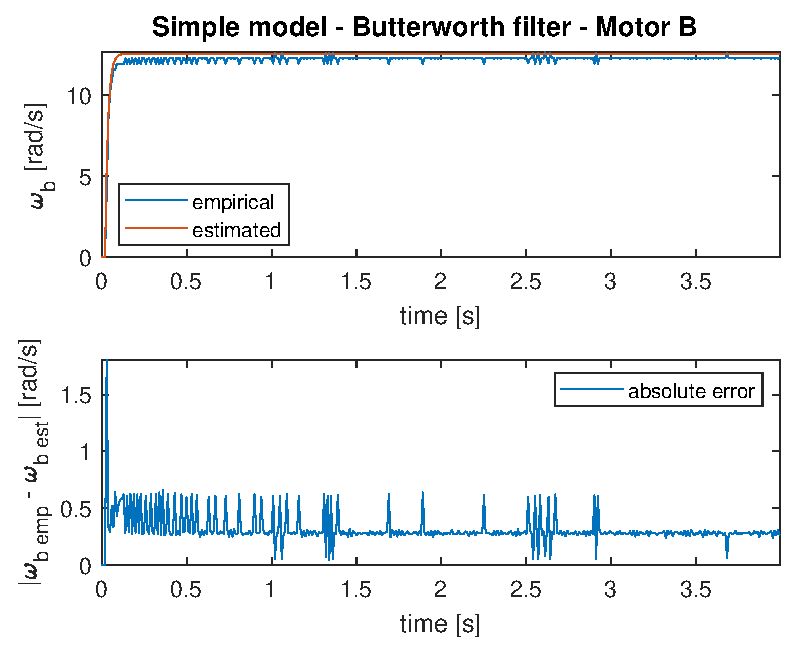
\includegraphics[width=\linewidth]{step_response_simple_BW_b.eps}
	\end{subfigure}
	\par\bigskip
	\begin{subfigure}[b]{0.48\textwidth}
		\centering
		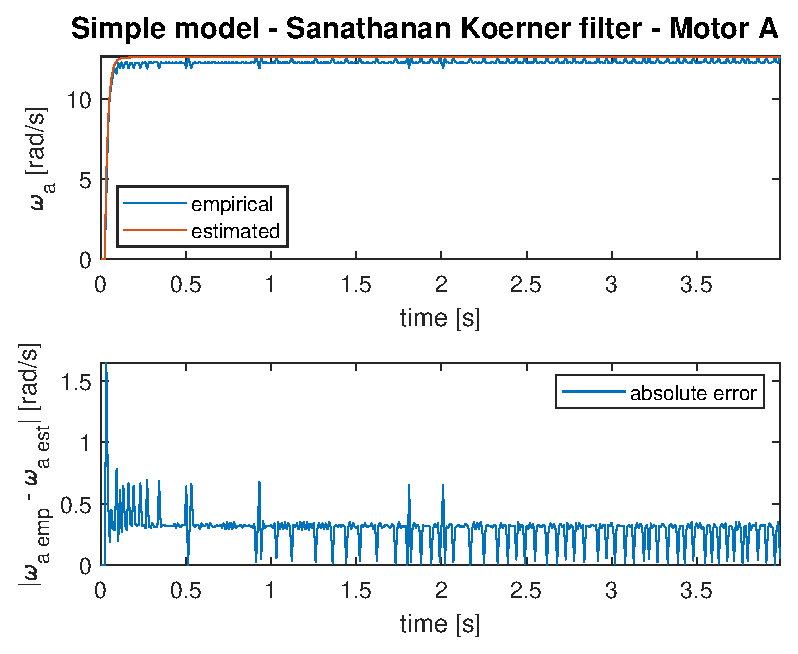
\includegraphics[width=\linewidth]{step_response_simple_SK_a.eps}
	\end{subfigure}
	\hfill
	\begin{subfigure}[b]{0.48\textwidth}
		\centering
		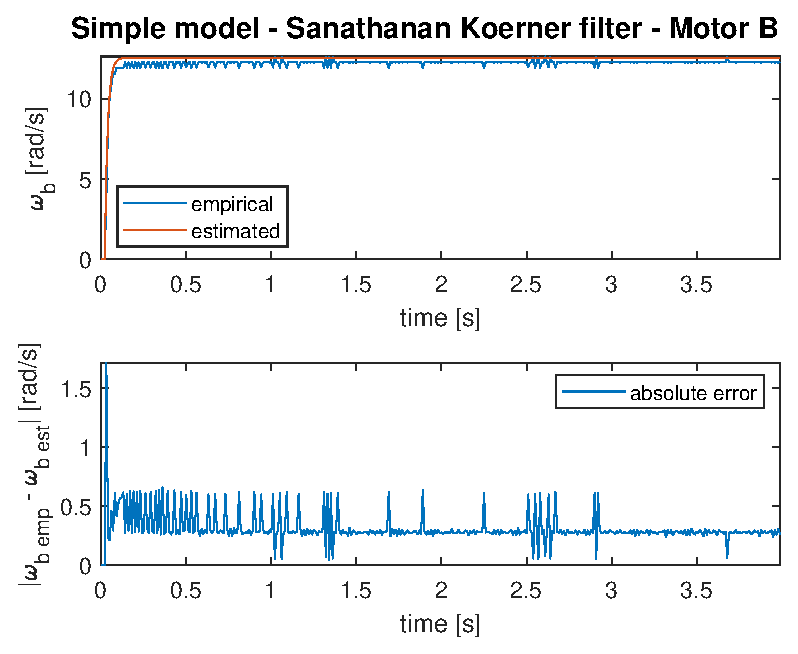
\includegraphics[width=\linewidth]{step_response_simple_SK_b.eps}
	\end{subfigure}
	\caption[Experimental results for the simple models]{Experimental results for the \textbf{simple} models: without filter, with Butterworth and with Sanathanan Koerner. The left side concerns motor A, while the right side concerns motor B. There are two types of plots: the top ones express the wheel velocity, while the bottom ones indicate the absolute error between the empirical wheel velocity and the velocity predicted by the model.}
	\label{fig:validation_simple}
\end{figure*}


\subsubsection{Superposition Principle}
The superposition principle system states that, for linear systems, the total response to a weighted sum of input signals is equal to the same weighted sum of the responses of the individual signals. In symbols:
\begin{equation}
\left.
\begin{split}
	u_1[t] \rightarrow y_1[t]\\
	u_2[t] \rightarrow y_2[t]
\end{split}
\quad
\right\}
\quad \Longrightarrow c_1 u_1[t] + c_2 u_2[t] \rightarrow c_1 y_1[t] + c_2 y_2[t]
\end{equation}
with $c_1, c_2$ arbitrary constants. To verify this, excitations of 4V, 6V and 10V are applied to the system. The excitation voltages of the 4V and the 6V measurement are summed and in Figure \ref{fig:superposition}, the sum of the individual wheel velocities is plotted. Next, the response of the system to the 10V excitation signal is plotted as well. If this would be a linear system, the superposition principle would be valid, so one would expect that these two graphs would more or less coincide. However, this is clearly not the case. The absolute error between these outputs is visualized as well. This error is too big to attribute to noise. Moreover, one would expect noise to have mean value equal to zero, which is clearly not the case. Conclusion: this system is non-linear. This non-linearity can be due to Coulomb friction in the motors, backlash of the gears, etc.


\begin{figure*}[htp!]
	\centering
	\begin{subfigure}[b]{0.48\textwidth}
		\centering
		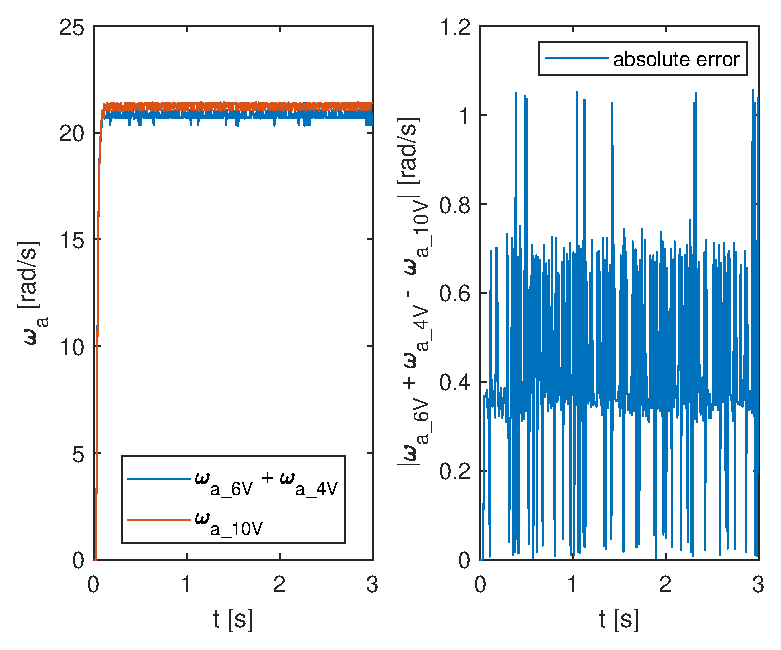
\includegraphics[width=\textwidth]{superposition_a.eps}
		\caption{Motor A}
	\end{subfigure}
	\hfill
	\begin{subfigure}[b]{0.48\textwidth}  
		\centering 
		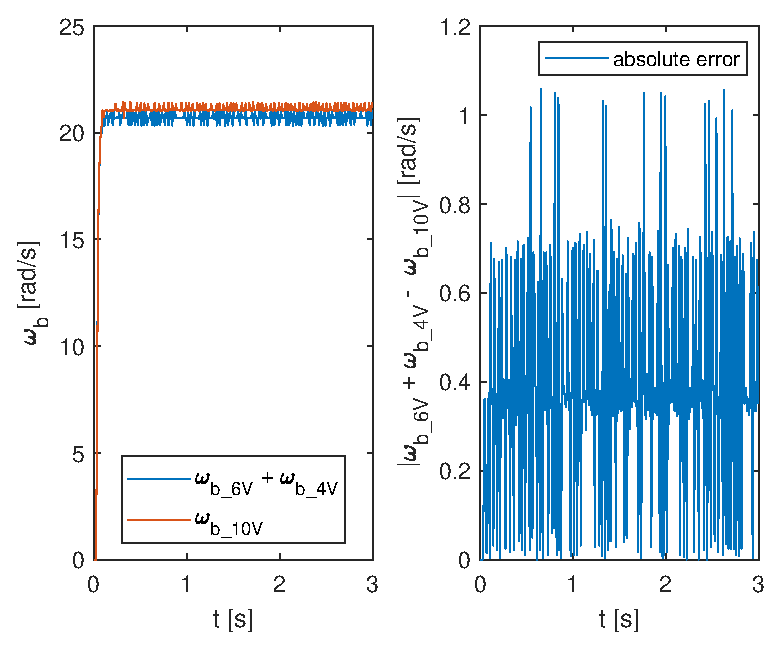
\includegraphics[width=\textwidth]{superposition_b.eps}
		\caption{Motor B}
	\end{subfigure}
	\caption[Superposition principle]{This system violates the superposition principle, as the blue and red curves do not coincide. For both motors, the right graph displays the absolute error between the response of the system to the sum of a 4V and 6V signal and the response to a 10V signal.} 
	\label{fig:superposition}
\end{figure*}


% ---------------------------------------------------------------------------
% ---------------------------------------------------------------------------

\section{Identification of the Cart on the Ground}

\subsection{Model Validation}



In this section, the cart is put on the ground. Figure \ref{fig:step_ground} depicts the measured response and the simulated response of the \textit{'old'} model selected in Subsection \ref{subsec:validation}, i.e. the simple, unfiltered model, when a step input is applied. The absolute error between these responses is also given for both motors.
\\\\
One can immediately observe that the estimated response is too fast. This is due to the fact that the inertia of the cart and the static friction of the wheels with the ground are not accounted for in the simple model. 




\begin{figure*}[htp!]
	\centering
	\begin{subfigure}[b]{0.49\textwidth}
		\centering
		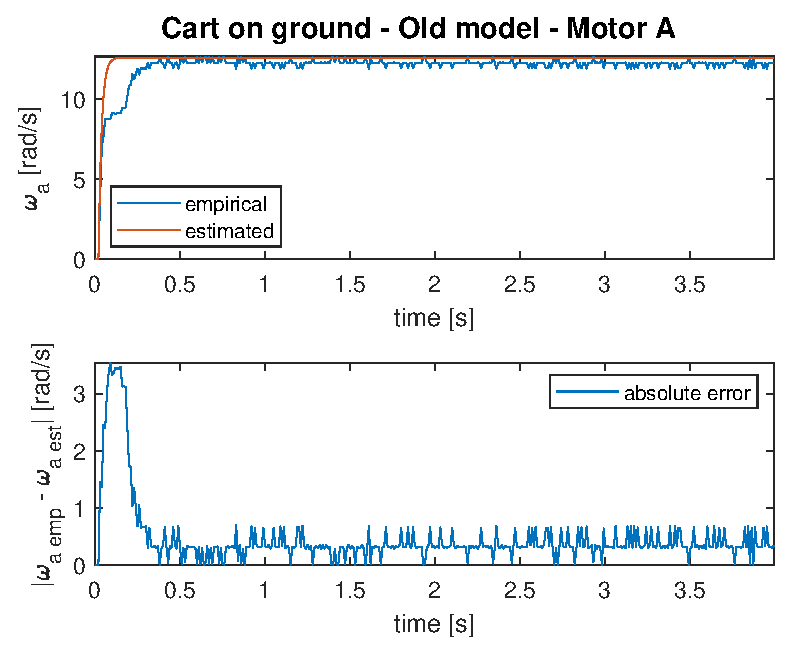
\includegraphics[width=\textwidth]{step_response_g_a.eps}
		\caption{Motor A}
	\end{subfigure}
	\hfill
	\begin{subfigure}[b]{0.49\textwidth}  
		\centering 
		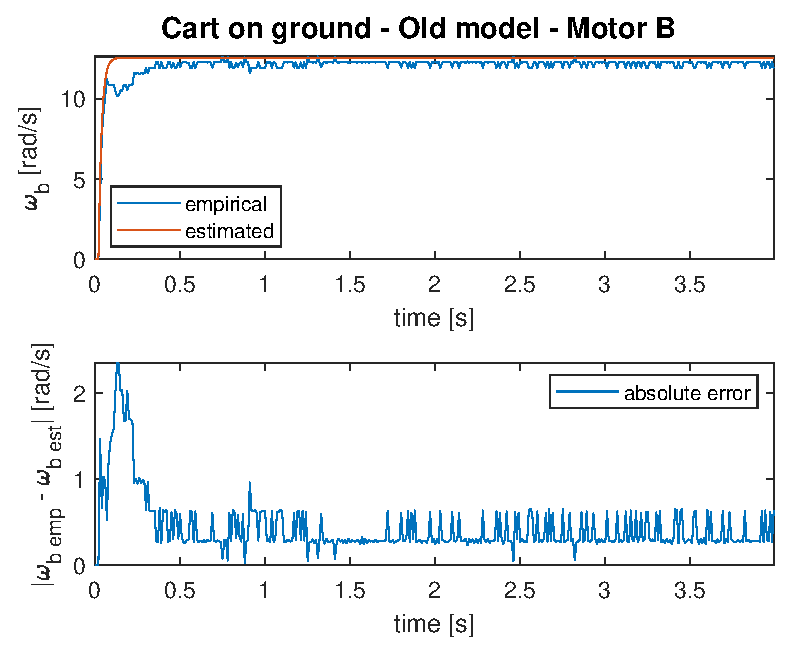
\includegraphics[width=\textwidth]{step_response_g_b.eps}
		\caption{Motor B}
	\end{subfigure}
	\caption[Cart on the ground, old model]{Empirical and simulated response of the \textbf{'old'} model when the cart that is placed on the ground and subject to a step excitation. The bottom graphs give the absolute error between these two.} 
	\label{fig:step_ground}
\end{figure*}

% ---------------------------------------------------------------------------

\subsection{Re-identification}

As it just turns out, it can be opportune to re-identify the models when the cart is placed on the ground. The results of this identification are found in Table \ref{tab:overview_re}. Furthermore, Figure \ref{fig:step_ground_new} depicts again the measured response and the simulated response of the \textit{'new'} model to a step input. 
\\\\
It is expected that the gain of the newly identified model is smaller, due to the friction of the wheels with the ground. This translates to a smaller value of $b_0$. Furthermore, one should also expect the poles to have a smaller frequency, due to the inertia of the cart. This matches bigger $a_0$ value.
\\\\
It suffices to compare Table \ref{tab:overview_re} to Table \ref{tab:overview} to see that both of these expectations are met. Conclusion: the newly identified model matches reality better. This is at last confirmed by the smaller absolute errors in Figure \ref{fig:step_ground_new}.


\begin{table}[htp]
	\centering
	\caption{Overview of the newly identified model for each motor.}
	\label{tab:overview_re}
	\bgroup
	\def\arraystretch{1.8}
	\begin{tabular}{|c||c|c|}
		\hline & \textbf{Motor A} & \textbf{Motor B}
		\\ \hline \hline
		Transfer function & \scalebox{1.15}{$\frac{ 0.5689}{z^2 - 0.7191\text{ }z}$} & \scalebox{1.15}{$\frac{ 0.6164}{z^2 - 0.6928\text{ }z}$}
		\\ \hline
		Poles [rad/s] & 33; NaN & 36.7; NaN
		\\ \hline
		Zeros [rad/s] & / & /
		\\ \hline
	\end{tabular}
	\egroup
\end{table}

\begin{figure*}[htp!]
	\centering
	\begin{subfigure}[b]{0.49\textwidth}
		\centering
		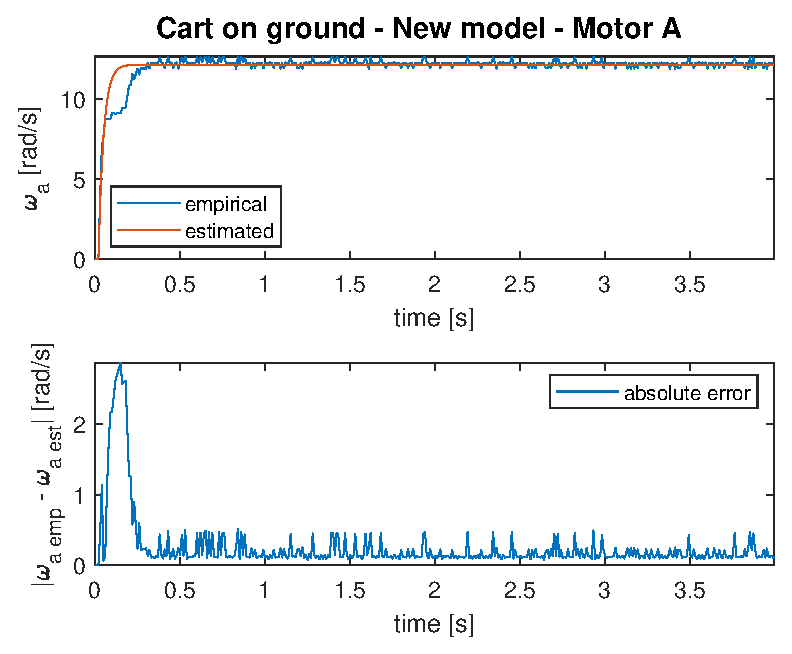
\includegraphics[width=\textwidth]{step_response_g_NF_a.eps}
		\caption{Motor A}
	\end{subfigure}
	\hfill
	\begin{subfigure}[b]{0.49\textwidth}  
		\centering 
		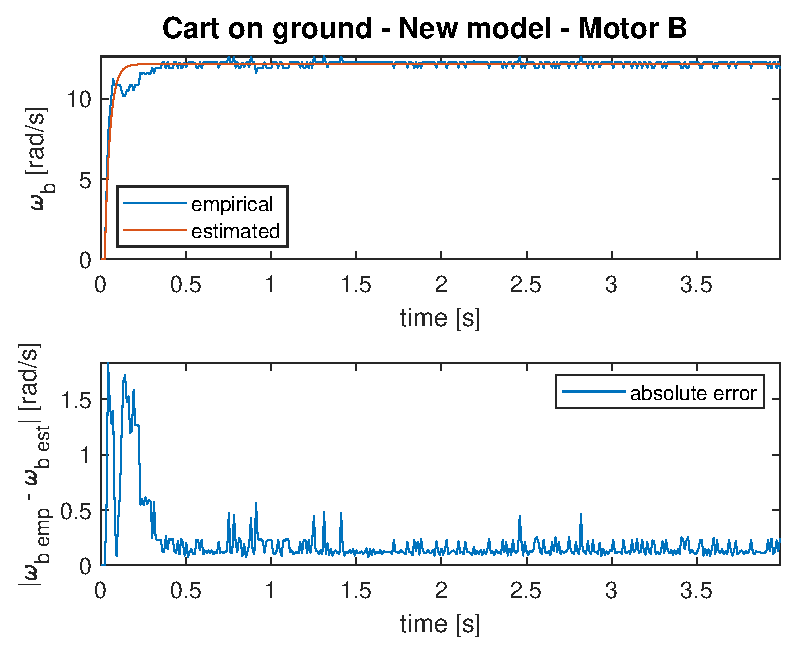
\includegraphics[width=\textwidth]{step_response_g_NF_b.eps}
		\caption{Motor B}
	\end{subfigure}
	\caption[Cart on the ground, new model]{Empirical and simulated response of the \textbf{'new'} model when the cart that is placed on the ground and subject to a step excitation. The bottom graphs give the absolute error between these two.} 
	\label{fig:step_ground_new}
\end{figure*}






\end{document}